\documentclass[openany]{book}

\usepackage{generalsnips}
\usepackage{calculussnips}
\usepackage[margin = 1in]{geometry}
\usepackage{pdfpages}
\usepackage[spanish]{babel}
\usepackage{amsmath}
\usepackage{amsthm}
\usepackage[utf8]{inputenc}
\usepackage{titlesec}
\usepackage{xpatch}
\usepackage{fancyhdr}
\usepackage{tikz}
\usepackage{hyperref}
\usepackage{supertabular}
\usepackage{float}
\pagestyle{empty}

\title{Summary on Teorías monetarias}
\begin{document}
\tableofcontents
%%%%%%%%%%%%%%%%%%%%%%%%%%%%%%%%%%%%%%%%%%%%%%%%%%%%%%%%%%%%%%%%%%%%%%%%%%%%%%%%%%%%%%%%%%%%%%%%%%%%%%%%%%%%%%%%%%%%%%%%%%%%%%%%%%%%%%%%%%%%%%

\chapter{Presentation 1}
\section{Production possibility frontier}
\begin{itemize}
    \item It's curved outward because of: 
        \begin{itemize}
            \item Law of diminishing marginal returns and law of increasing opportunity cost. 
        \end{itemize}
    
    \item Tom and Jen: 
        \begin{itemize}
            \item Specialization, are when each individual dedicates all of his time and resources on producing the thing that has the less opportunity cost. 
            \item All combinations that are without specialization are less than potential. 
        \end{itemize}
\end{itemize}

\section{Economic freedom }
Economic freedom means: 
\begin{itemize}
    \item Property rights 
    \item Freedom to exchange 
    \item Give their property willingly 
    \item All of this only if their actions don't violate other peoples' liberties. 
\end{itemize}
To achieve high economic freedom: 
\begin{itemize}
    \item Keep government spending and taxes low
    \item Sound money 
    \item Property rights 
    \item Enforce contracts evenhandedly 
    \item Refrain from imposing trade barriers 
\end{itemize}

\section{Five areas of EFW Index}
\begin{enumerate}
    \item Size of government 
    \item Legal system and protection of property rights 
    \item Access to sound money 
    \item Freedom to trade internationally 
    \item Regulation of capital, labor and business (my freedom to do whatever with whats mine)
\end{enumerate}

\section{Three lessons from the EFW}
\begin{enumerate}
    \item Economic freedom has increased since 1980.
    \item Income gap between high-income and developing countries has narrowed.
    \item Economic freedom matters, high economic freedom means high GDP, rapid growth. 
\end{enumerate}



%%%%%%%%%%%%%%%%%%%%%%%%%%%%%%%%%%%%%%%%%%%%%%%%%%%%%%%%%%%%%%%%%%%%%%%%%%%%%%%%%%%%%%%%%%
\chapter{Presentation 2}
\section{Stock and flow variables}
\begin{itemize}
    \item Stock: una variable que se acumula (riqueza de la nación).
    \item Flows: es una variable que se reinicia cuando termina un periodo. (GDP) se puede medir en un periodo de tiempo.
\end{itemize}

\section{Macroeconomic goals, framework, and policies}
Goals: the most important objectives for the macro economy. 
\begin{itemize}
    \item Economic growth: increment in real GDP.
    \item Low unemployment: rate of unemployment is equal to the natural rate of unemployment $\approx$ 5\%
    \item Low and stable inflation: more important for it to be stable.
\end{itemize}
Framework: used to analyze macroeconomic changes. 
\begin{itemize}
    \item Aggregate demand / aggregate supply
    \item Keynesian model
    \item Neoclassical model 
\end{itemize}
Policy tools: tools of the government and central bank to influence money. 
\begin{itemize}
    \item Monetary policy: printing money, supplying money, policy on monetary multiplier (RRr), these policies control inflation. 
        \begin{itemize}
            \item Central bank 
            \item $\Delta m_2$ 
        \end{itemize}
    \item Fiscal policy: policy related to taxes and government spending.
        \begin{itemize}
            \item Taxes and government spending
            \item G $>$ T: deficit 
        \end{itemize}
\end{itemize}

\section{GDP}
\begin{itemize}
    \item Gross Domestic Product (GDP): dollar value of all output of all goods and services produced \textbf{within} a countries borders. 
    \item An economy's GDP can be measured (they both have to be equal, if there is a difference it's because of the informal sector): 
        \begin{itemize}
            \item Total dollar value of what consumers \textbf{purchase}, expenditure approach.
            \item Total dollar value of what a country \textbf{produces} income approach.
            \item Value added approach (gross value of output - value of intermediate consumption)
        \end{itemize}
\end{itemize}

\section{GDP Measured by components of demand (expenditure approach)}
\begin{itemize}
    \item The consumer buys all the country's production.
    \item Demand for production can be divided into four main parts: 
        \begin{itemize}
            \item Consumer spending (consumption)
            \item Business spending (investment)
            \item Government spending on goods and services
            \item Spending on net exports 
        \end{itemize}
\end{itemize}

\subsection{New export component}
\begin{itemize}
    \item Trade balance: gap between exports and imports.
        \[
            \text{ Trade balance } = \p{X - M} 
        \]
    \item Trade surplus: exports $>$ imports, positive quantity. 
    \item Trade deficit: exports $<$ imports, negative quantity. 
\end{itemize}

\subsection{GDP Using demand}
\[
  \text{ GDP } = \text{ Consumption } + \text{ Investment } + \text{ Government } + \text{ Trade balance }
\]
\[
  \text{ GDP } = C + I + G + (X-M)
\]


\section{GDP measured by what is produced (income approach)}
Because every transaction must have a buyer and a seller. 
\begin{itemize}
    \item Durable goods 
    \item Non-durable goods
    \item Services 
    \item Structures 
    \item Change in inventories 
\end{itemize}
\[
  \text{ Income approach } = \text{ Total national income } + \text{ Sales taxes } + \text{ Net foreign income }
\]

\section{GNP and NNP}
\begin{itemize}
    \item Gross National Product (GNP): it's GDP + Business abroad. 
    \item Net National Income (NNP): GNP - depreciation
    \item NNP 
\end{itemize}
%
\section{Real GDP vs Nominal GDP}
\begin{itemize}
    \item Real GDP: GDP after it has been adjusted for inflation 
    \item Nominal GDP: GDP announced at the time, not adjusted for inflation. 
\end{itemize}
%
\subsection{GDP Deflator}
\begin{itemize}
    \item GDP deflator is a price index calculated by the average price of all goods and services in an economy (it's the ratio of nominal and real GDP, also called price index)
\end{itemize}
Real GDP: 
\[
    \text{ Real GDP } = \frac{\text{ Nominal GDP }}{\cfrac{\text{ GDP Deflator }}{100}} 
\]

\section{GDP over time}
\begin{itemize}
    \item Recession: a significant decline in national output / GDP
    \item Depression: lengthy and deep decline in output. 
\end{itemize}

\section{Patterns of recessions and expansions}
\begin{itemize}
    \item Order: Peak $\rightarrow$ Recession $\rightarrow$ Trough $\rightarrow$ Expansion. 
    \item Business cycle: the economy's short term movement in and out of recession. 
\end{itemize}

\section{Comparing GDP among countries}
\begin{itemize}
    \item Exchange rate: value of one currency in terms of another. 
\end{itemize}
\[
    \text{ Brazil's GDP in \$U.S } = \frac{\text{ Brazils GDP in reals }}{\text{ Exchange rate (reals to USD) }} 
\]

\section{GDP per capita}
\[
  \text{ GDP per capita } = \frac{\text{ GDP }}{\text{ Population }} 
\]

\section{How well GDP measures the well-being of society}
\begin{itemize}
    \item GDP isn't good for measuring happiness nor standard of living but it's the closest thing we've got to measure. 
    \item Standard of living: all elements that affect people’s happiness and well-being, whether they are bought and sold in the market or not.
\end{itemize}
GDP vs standard of living, GDP doesn't include a lot: 
\begin{itemize}
    \item Leisure time 
    \item Environmental cleanliness, health and learning 
    \item Production not exchange in the market 
    \item Level of inequality
    \item Technologies and availability of products. 
\end{itemize}

%%%%%%%%%%%%%%%%%%%%%%%%%%%%%%%%%%%%%%%%%%%%%%%%%%%%%%%%%%%%%%%%%%%%%%%%%%%%%%%%%%%%%%%%%%
\chapter{Presentation 3}
\section{Unemployment rate}
\begin{itemize}
    \item Employed: Currently working 
    \item Unemployed: out of work and actively looking for a job.
    \item Labor force = Employed + Unemployed 
    \item Unemplyment rate: 
        \[
          \text{ Unemployment rate } = \frac{\text{ Unemployed people }}{\text{ Total labor force }} \times 100 
        \]
\end{itemize}

\subsection{Hidden unemployment}
Mislabeled people: 
\begin{itemize}
    \item Part-time: temporary.
    \item Underemployed: economist working at mc donald's.
    \item Discouraged workers: those who have stopped looking for employment due to the lack of suitable positions available.
    \item *Extra Transition: person who quits their job to go to another one. 
\end{itemize}

\subsection{Labor force participation}
Labor force participation rate: in proportion to all adults in a country how many people are in the labor force (can work). 
\[
  \text{ Labor force participation rate } = \frac{\text{ Total labor force }}{\text{ Total adult population }} \times 100
\]

\subsection{Patterns of unemployment}
Unemployment moves up and down as the economy moves in and out of recessions and business cycles.

\section{Unemployment facts}
\begin{itemize}
    \item Unemployment in a gender comparison are relatively equal, and they used to be lower for men. 
    \item Unemployment tends to be higher in ages 16-19.
\end{itemize}


%----------------------------------------------------------------------------------------
\section{Cyclical unemployment}
\begin{itemize}
    \item Cyclical unemployment: closely related to the business cycle, higher unemployment during a recession is cyclical unemployment. 
\end{itemize}


%----------------------------------------------------------------------------------------
\section{Unemployment and equilibrium in the labor market}
\begin{itemize}
    \item Labor market is the same as any other market with the subtle difference of the y-axis having wage rate and the x-axis having Quantity of labor. 
\end{itemize}

\subsection{Sticky wages}
\begin{itemize}
    \item The minimum wage creates sticky wages above the equilibrium. 
\end{itemize}


%----------------------------------------------------------------------------------------
\section{Changes in unemployment on the long run}
Natural rate of unemployment: 
\begin{itemize}
    \item Frictional unemployment: unemployment ``between jobs''.
    \item Structural unemployment: individuals lack skills valued by employers thus they are unemployed. 
\end{itemize}
Full unemployment: when the unemployment rate is equal to the natural unemployment rate. 

\subsection{Productivity shifts and the natural rate of unemployment}
\begin{itemize}
    \item At some point the wage rate (based on productivity) will be grater than the demand of labor (grater than the optimal point).
    \item This increase in wage and demand will eventually create unemployment. 
\end{itemize}

\chapter{Presentation 4}
\section{Tracking inflation}
\begin{itemize}
    \item Inflation: general rise in the level of prices in an entire economy.  
    \item Basket of goods and services: hypothetical group of items, with specified quantities of each one meant to represent a ``typical'' set of consumer purchases.
        \begin{itemize}
            \item Used to calculate price levels. 
        \end{itemize}
\end{itemize}

%----------------------------------------------------------------------------------------
\section{Index Numbers}
\begin{itemize}
    \item Index number: a unit-free number derived from the price level over a number of years, which makes computing inflation rates easier, since the index number has values around 100.
        \begin{itemize}
            \item It doesn't have any unit.
        \end{itemize}
    \item Base year: arbitrary year whose value as an index number economists define as 100.
\end{itemize}
Inflation: 
\[
  \text{ Inflation rate  }(\pi) = \frac{\p{\text{ Price Level in new year } - \text{ Price Level in prior year }} }{\text{ Level in prior year }} \times 100
\]

%----------------------------------------------------------------------------------------
\section{Measure changes in the cost of living}
\begin{itemize}
    \item Consumer price index (CPI): to measure inflation government statisticians calculate based on the price level from a fixed basket of goods and services that represent an average consumer's purchases. 
    \item Substitution bias: n inflation rate calculated using a fixed basket of goods over time tends to overstate the true rise in the cost of living, becuase it doesn't take into account that the person can substitute away from goods whose prices rise considerably. 
    \item Quality / new goods bias:  inflation calculate using a fixed basket of goods over time tends to overstate the true rise in cost of living, because it doesn't account for improvements in the quality of existing goods or the invention of new goods. 
\end{itemize}

\section{Additional price indices}
\begin{itemize}
    \item Producers Price Index (PPI): a measure of inflation based on prices paid for supplies and inputs by producers of goods and services. 
    \item Internationl price index: a measure of inflation based on the prices of merchandise that are exported or imported. 
    \item Employment cost index: measure of inflation based on wages paid in the labor market.
    \item GDP deflator: a measure of inflation based on the prices of all the GDP components. 
\end{itemize}


%----------------------------------------------------------------------------------------
\section{The confusion over inflation}
\begin{itemize}
    \item The problem with inflation is that it doesn't sync in real time to measurements, this causes economic problems:
    \begin{itemize}
            \item Unintended redistributions of purchasing power.
            \item Blurred price signals. 
            \item Difficulties in long-term planning.  
        \end{itemize}    
    \item There is a time lag in prices, wages and interest rates. 
\end{itemize}



%----------------------------------------------------------------------------------------
\section{Indexing and its limitations}
\begin{itemize}
    \item Indexed - a price, wage, or interest rate is adjusted automatically for inflation.
    \item Cost of living adjustments (COLAs): wages increase as inflation increases. 
    \item Adjustable-rate mortgage (ARM): a type of loan a borrower uses to purchase a home in which the interest rate varies with market interest rates. 
\end{itemize}
%----------------------------------------------------------------------------------------
\section{Real interest rate}
Real interest paid (Fischer equation): 
\[
  i_{rt} = r - \pi  
\]
\begin{itemize}
    \item $i_{rt}$ Long term nominal interest rate 
    \item $r$: Nominal interest rate 
    \item $\pi$: actual or expected rate of inflation or deflation
\end{itemize}


%%%%%%%%%%%%%%%%%%%%%%%%%%%%%%%%%%%%%%%%%%%%%%%%%%%%%%%%%%%%%%%%%%%%%%%%%%%%%%%%%%%%%%%%%%
\chapter{Presentation 5}
\section{Functions of money}
Before money, we had: 
\begin{itemize}
    \item Barter: trading one good or service for another (without using money).
    \item Double coincidence of wants: situation of one individual wanting one good or service that the other can provide. 
\end{itemize}
Money serves: 
\begin{itemize}
    \item Medium of exchange: generally accepted as payment.
    \item Store of value: preserves economic value across time.
    \item Unit of account: common way to measure value. 
    \item Standard of deferred payment: acceptable in the future.
\end{itemize}

\section{Commodity vs Fiat money}
\begin{itemize}
    \item Commodity money: item used for money but can also serve as something other than money. 
    \item Commodity-backed currencies: currency backed by other commodity such as gold. 
    \item Fiat money: has n intrinsic value, declared by a country as legal tender. Meaning the only thing backing our money is faith and trust. 
\end{itemize}

\section{Measuring money: currency M1 and M2}
Central bank: 
\begin{itemize}
    \item The federal reserve 
    \item Bank regulator and responsible for monetary policy. 
    \item Defines money according to its liquidity. 
\end{itemize}
Two definitions of money: 
\begin{itemize}
    \item M1 money supply (Medio circulante): currency in circulation + checkable (demand) accounts + traveler's checks
        \begin{itemize}
            \item Currency in circulation: currency circulating in an economy not held at the Treasury, the central bank, or the bank vaults.
            \item Checkable (demand) deposits: checkable deposit in banks that is available by making a cash withdrawal or writing a check.
        \end{itemize}
    \item M2 money supply: M1 + savings deposits + money market funds + certificates of deposit + other time deposits
        \begin{itemize}
            \item Saving deposits: savings, not easily transferable to cash. 
            \item Money market fund: deposits of many investors to be invested in projects. (They are secure investments)
            \item Certificates of deposit: leave your money in a bank but you can't withdraw it for a period of time. 
        \end{itemize}
\end{itemize}

%----------------------------------------------------------------------------------------
\section{How do banks make profit}
\begin{itemize}
    \item Financial intermediary: an institution that operates between a saver with financial assets to invest and an entity who will borrow those assets and pay a rate of return. (banks stand between savers and borrowers)
    \item Deposit institution: institution that accepts money deposits and then uses these to make loans.
\end{itemize}
For the bank: a loan is an asset, a deposit is a liability. Banks balance sheet: 
\begin{center}
    \begin{tabular}{ |p{6cm}|p{6cm}| }
        \hline
            Assets & Liabilities + Net worth  \\
        \hline
            \begin{itemize}
                \item Loans 
                \item Government securities 
                \item Reserves 
            \end{itemize}
            & 
            \begin{itemize}
                \item Deposits 
                \item Net worth (assets - liabilities)
            \end{itemize}
            \\ 
        \hline
    \end{tabular}
\end{center}

%----------------------------------------------------------------------------------------
\section{Reserves and bankruptcy}
\begin{itemize}
    \item Reserves: funds that a bank keeps on hand and that it does not loan out or invest in bonds.
\end{itemize}


%----------------------------------------------------------------------------------------
\section{How banks go bankrupt}
\begin{itemize}
    \item High rate of loan defaults 
    \item Asset-liability time mismatch: we all go to the bank at once.
\end{itemize}
To reduce risk: 
\begin{itemize}
    \item Diversify: loans to a lot of people (don't have all your eggs in the same basket).
    \item Sell loans in a secondary loan market 
    \item Hold a greater share of assets (government bonds or reserves)
\end{itemize}

\section{Banks create money}
\begin{itemize}
    \item The monetary multiplier depends on the fraction of the reserve they are obligated to keep.
\end{itemize}
Monetary multiplier: 
\[
  \text{ Monetary multiplier formula } = \frac{1}{\text{ Reserved Requirement }} 
\]
\begin{itemize}
    \item This formula is the supply of money created by the banking system, how many times money can be multiplied.
\end{itemize}
For calculating the total money created: 
\[
  \text{ Total Money Created } = \text{ Monetary multiplier } \times \text{ Excess reserves }
\]

%----------------------------------------------------------------------------------------
\subsection{Cautions about the money multiplier}
Banks may decide to vary how much they hold in reserves for two reasons: 
\begin{itemize}
    \item Macroeconomic conditions 
    \item Government rules 
\end{itemize}
Cautions:
\begin{itemize}
    \item Banks usually hold more reserves do to greater uncertainty. 
    \item Federal reserves can raise or lower reserve ratio. 
\end{itemize}


%%%%%%%%%%%%%%%%%%%%%%%%%%%%%%%%%%%%%%%%%%%%%%%%%%%%%%%%%%%%%%%%%%%%%%%%%%%%%%%%%%%%%%%%%%
\chapter{Presentation 7}
%----------------------------------------------------------------------------------------
\section{Central bank of Guatemala}
\subsection{Bank structure}
\begin{itemize}
    \item Objective: garantizar la estabilidad monetaria, cambiaraia y crediticia del pais.
    \item Governed by the ``Junta Monetaria''
\end{itemize}

%%%%%%%%%%%%%%%%%%%%%%%%%%%%%%%%%%%%%%%%%%%%%%%%%%%%%%%%%%%%%%%%%%%%%%%%%%%%%%%%%%%%%%%%%%

\chapter{Video Review}
\section{Determinants of worker productivity} 
\begin{itemize}
    \item Human capital: accumulated knowledge, skill, and expertise that the average worker in an economy possesses. 
    \item Technological change: a combination of invention and innovation.
        \begin{itemize}
            \item Invention - advances in knowledge 
            \item Innovation - putting advances in knowledge to use in a new product or service.
        \end{itemize}
    \item Economy of scale: the cost advantages that industries obtain due to size. 
\end{itemize}

\section{Sources of economic growth}
\begin{itemize}
    \item Production function: the process whereby a firm turns economic inputs like labor, machinery, and raw material into outputs like goods and services that consumers use.
    \item Aggregate production function: the process whereby an economy as a whole turns economic inputs such as human capital, physical capital, and technology into output measured as GDP per capita. 
    \item In macroeconomics, we call the connection from inputs to outputs for the entire economy an aggregate production function.
    \item Growth of productivity is linked to GDP per capita.
\end{itemize}

\section{Funding investment}
\[
  \underbrace{I}_{\text{ US Capital }} = \underbrace{S}_{\text{ Private saving }} + \underbrace{(T-G)}_{\text{ Government saving }} + \underbrace{(IM-EX)}_{\text{ Foreign saving }}
\]

\section{Three tools of central bank to $\Delta m2$ }
\begin{enumerate}
    \item $\Delta$RRr $\downarrow$RRd $\rightarrow$ $\uparrow $m2
    \item $\Delta$ discount rate 
        \begin{itemize}
            \item Interest rate the central bank charges banks for loans. 
            \item $\downarrow $ discount rate $\rightarrow$ $\uparrow $m2
            \item Open market operations 
                \begin{itemize}
                    \item Buying or selling of bonds.
                \end{itemize}
        \end{itemize}
\end{enumerate}

%----------------------------------------------------------------------------------------
\chapter{Quiz}
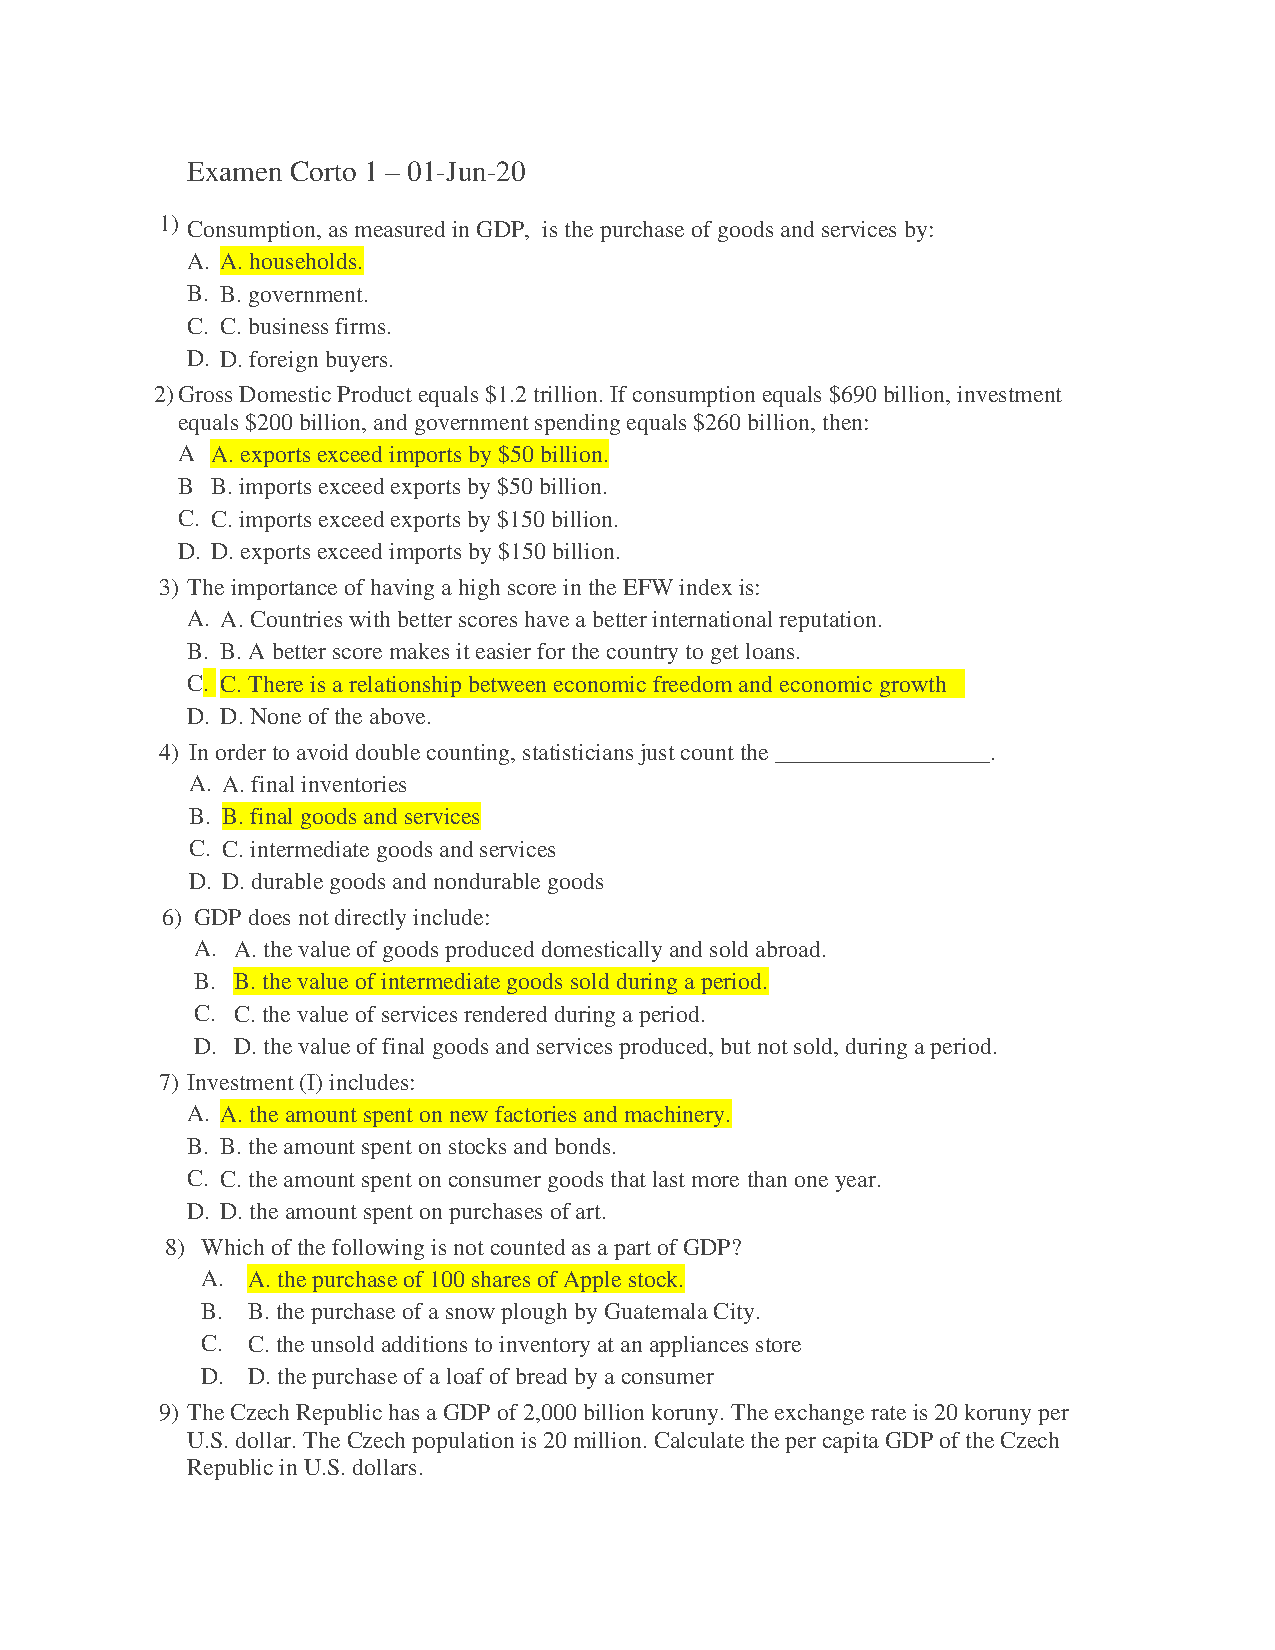
\includepdf[pages=-,pagecommand={\thispagestyle{empty}}]{figs/EC_01.pdf}
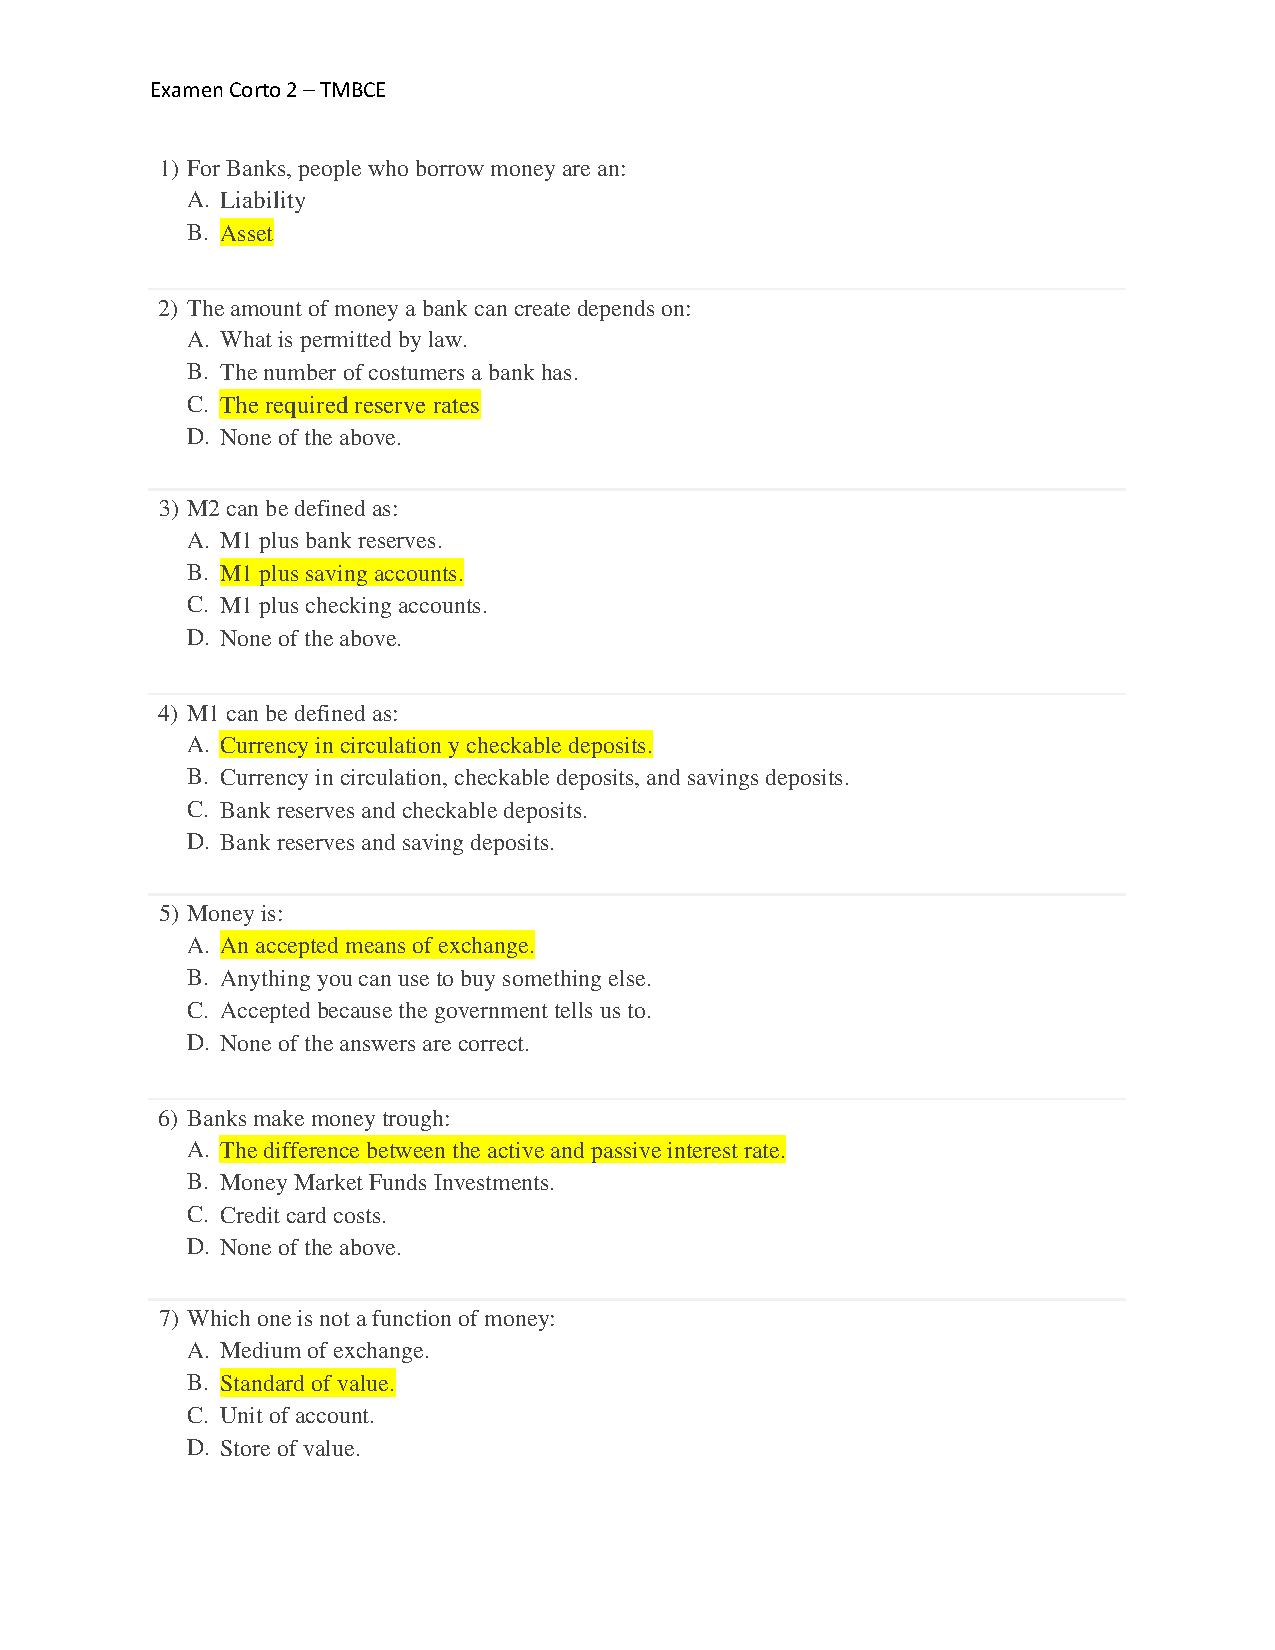
\includepdf[pages=-,pagecommand={\thispagestyle{empty}}]{figs/EC_02.pdf}

\includepdf[pages=-,pagecommand={\thispagestyle{empty}}]{figs/Tarea02-DavidCorzo-20190432.pdf}

%%%%%%%%%%%%%%%%%%%%%%%%%%%%%%%%%%%%%%%%%%%%%%%%%%%%%%%%%%%%%%%%%%%%%%%%%%%%%%%%%%%%%%%%%%
\chapter{Formulary}
\begin{center}
    \begin{supertabular}{ |p{16cm}| }
        \hline
            1 billon = 0.001 million \\ 
        \hline
            \[
                \text{ GDP } = C + I + G + (X-M)
            \] \\
        \hline
            \[
                \text{ Trade balance } = \p{X - M} 
            \] \\
        \hline
            \[
                \text{ Real GDP } = \frac{\text{ Nominal GDP }}{\cfrac{\text{ GDP Deflator }}{100}} 
            \] \\
        \hline
            \[
                \text{ Unemployment rate } = \frac{\text{ Unemployed people }}{\text{ Total labor force }} \times 100 
            \] \\
        \hline
            \[
                \text{ Labor force participation rate } = \frac{\text{ Total labor force }}{\text{ Total adult population }} \times 100
            \] \\
        \hline
        Inflation: 
            \[
                \text{ Inflation rate }(\pi) = \frac{\p{\text{Price Level in new year } - \text{Price Level in prior year }} }{\text{ Level in prior year }} \times 100
            \] \\
        \hline
            \[ 
                i_{rt} = r - \pi  
            \] \\ 
        \hline
        \[
            \text{ Monetary multiplier formula } = \frac{1}{\text{ Reserved Requirement }} 
        \] \\
        \hline
        \[
          \text{ Total Money Created } = \text{ Monetary multiplier } \times \text{ Excess reserves }
        \] \\
        \hline
        RGDP con el base year y price level. 
        \[
          RGDP^{19} = \sum_{i=0}^{n}P_{i}^{14} Q_{i}^{19}
        \] \\ 
        \hline 
        Productivity:  
        \[
            \text{ Productivity } = \frac{\text{ \#Output }}{\text{ \#Input }} 
        \] \\ 
        \hline
        Equation of exchange: 
        \[
          P_L \cdot \text{ RGDP } = \underbrace{m}_{\text{ Money supply }} \cdot \underbrace{v}_{\text{ Velocity average a dollar is spent }}
        \] \begin{itemize}
            \item Bitcoin has a fixed money supply thus $m$ is zero. 
        \end{itemize}\\ 
        \hline
        Nominal GDP: 
        \[
          \text{NGDP} = P_L \cdot \text{ RGDP }
        \] \\ 
        \hline
    \end{supertabular}
\end{center}


%%%%%%%%%%%%%%%%%%%%%%%%%%%%%%%%%%%%%%%%%%%%%%%%%%%%%%%%%%%%%%%%%%%%%%%%%%%%%%%%%%%%%%%%%%
\chapter{Figures}
\begin{figure}[H]
    \centering
    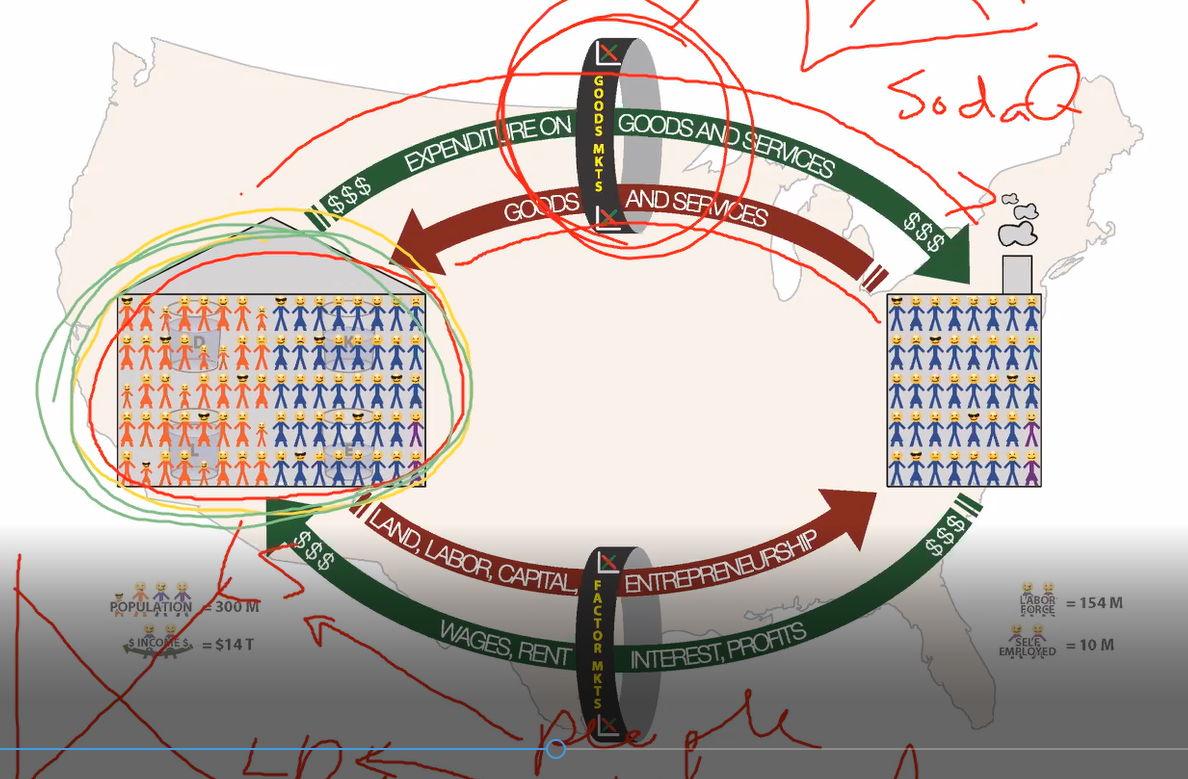
\includegraphics[width=14cm]{figs/Captura.PNG} 
\end{figure}
\begin{figure}[H]
    \centering
    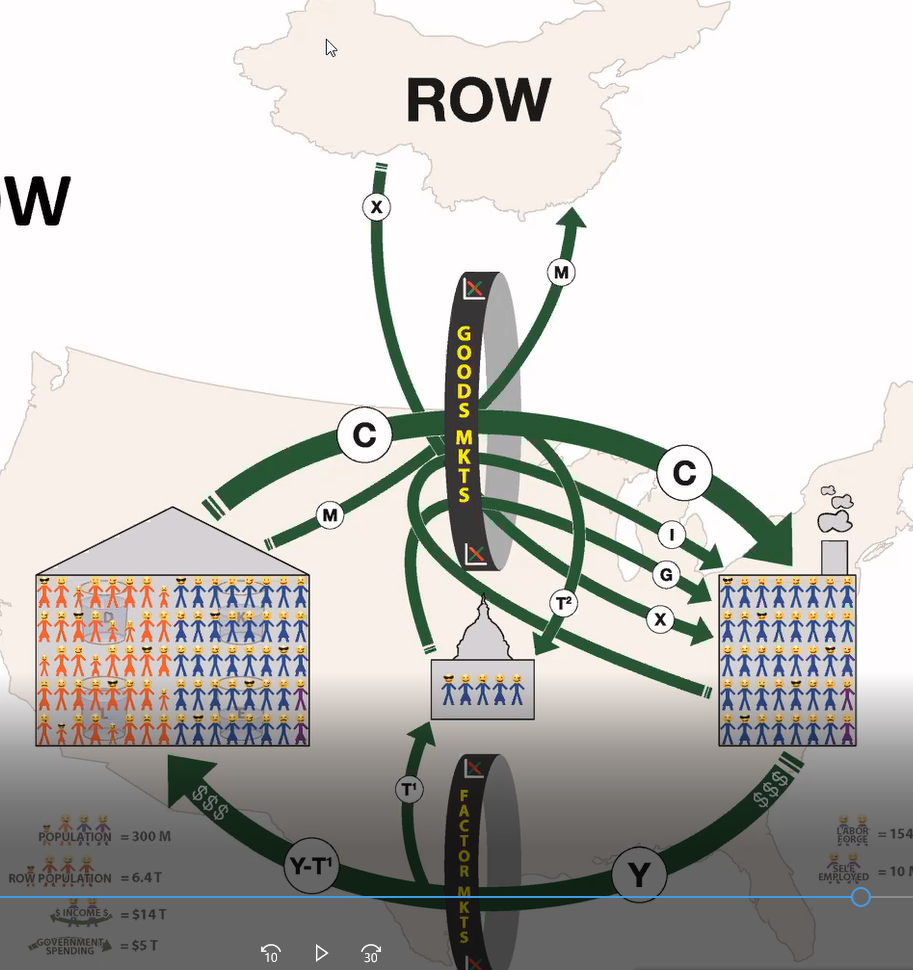
\includegraphics[width=14cm]{figs/Captura1.PNG}  
\end{figure}
\begin{figure}[H]
    \centering
    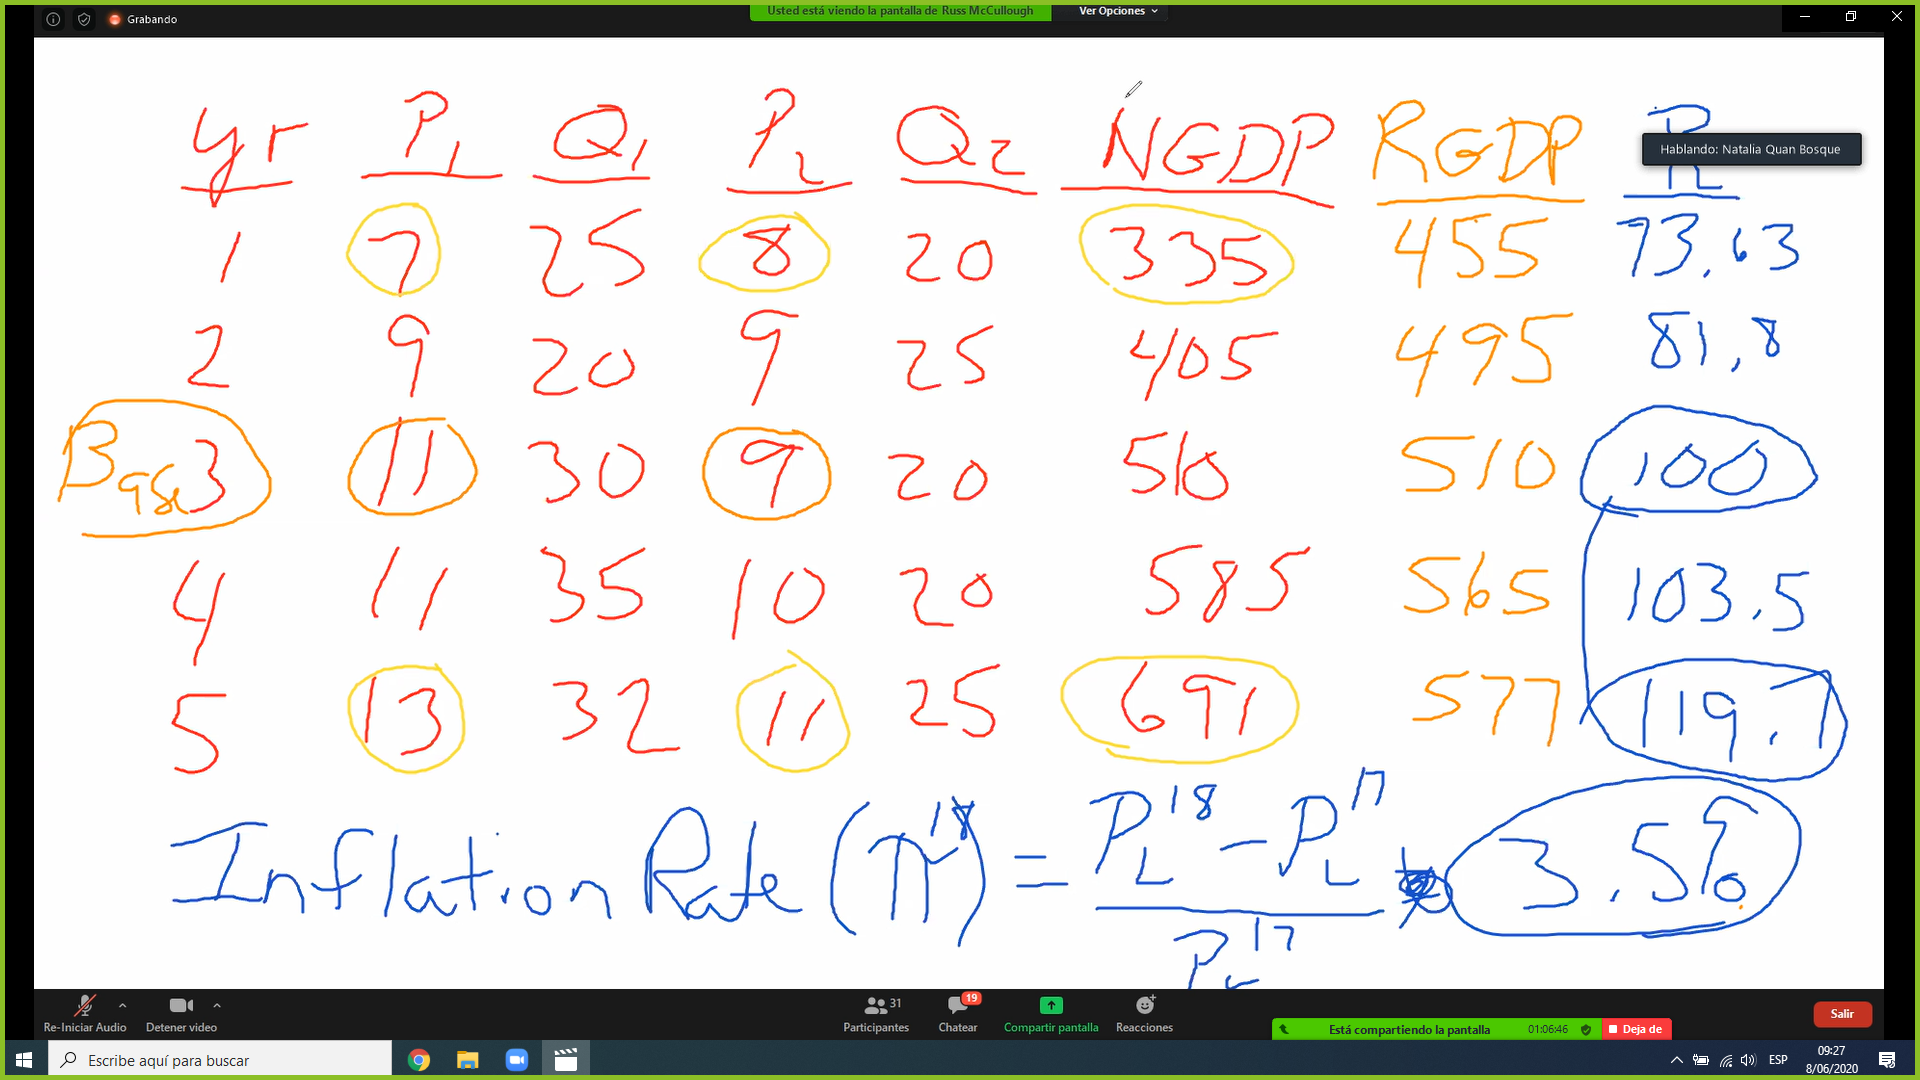
\includegraphics[width=14cm]{figs/Captura2.png} 
\end{figure}




%%%%%%%%%%%%%%%%%%%%%%%%%%%%%%%%%%%%%%%%%%%%%%%%%%%%%%%%%%%%%%%%%%%%%%%%%%%%%%%%%%%%%%%%%%%%%%%%%%%%%%%%%%%%%%%%%%%%%%%%%%%%%%%%%%%%%%%%%%%%%%
\end{document}

